\section{Progressive-Adaptive Music Generator for Videogames}

The last approach hence of adaptive and generative music
was published in 2023 by Alvaro Eduardo Lopez Duarte \cite{lopez2023progressive}.
It was developed to generate music for 
video games in real-time \cite{lopez2023progressive}.
The system of Lopez can be categorized in various categories of generative music \cite{lopez2023progressive}. It takes on the role of composing and arranging by creating new pieces of music and recombining existing melody lines and chords \cite{lopez2023progressive}. It also adapts the interpretation by changing parameters \cite{lopez2023progressive}. PAMG manages both the horizontal (temporal sequences) and vertical (simultaneous musical events) directions in the music \cite{lopez2023progressive}. It works at different levels of granularity such as phrases, bars, beats, notes and chords and uses a coarse grid as the minimum event duration, with the exception of arpeggios, ratchets and staccato events \cite{lopez2023progressive}.

In gameplay context, the music of the author's PAMG is non-
diegetic, which means it is not generated within the game 
world,
instead it belongs to the narrative representation of the
game \cite{lopez2023progressive}. The music within the game is ambient, that means it is
not tied to a specific source, and adaptive, as it changes 
based on game variables \cite{lopez2023progressive}. However, PAMG can also make changes
autonomously \cite{lopez2023progressive}.

The system consists of several agents, which are able to
adapt and create melodies, harmonies and rhythms 
\cite{lopez2023progressive}. The main components of 
the system are the Melody Agent, the Harmony Agent, the 
Percussion Agent and the Orchestrator Agent
\cite{lopez2023progressive}. The Melody Agent creates
and manages melodies, the Harmony Agent takes care of
the harmonies and chords, the Percussion Agent takes care
of rhytmic Elements and the Orchestrator Agent assigns
instruments families and makes real-time decisions on the
instrument usage \cite{lopez2023progressive}. Next to those
agents, a Multi-Parameter Preset Interpolator and Controller
(MPIC) enables control and interpolation between different 
presets, allowing smooth transitions between different 
musical settings \cite{lopez2023progressive}. The descripted
algorithm process can be seen in \Cref{fig:pamg_algorithm}

\begin{figure}[h]
    \centering
    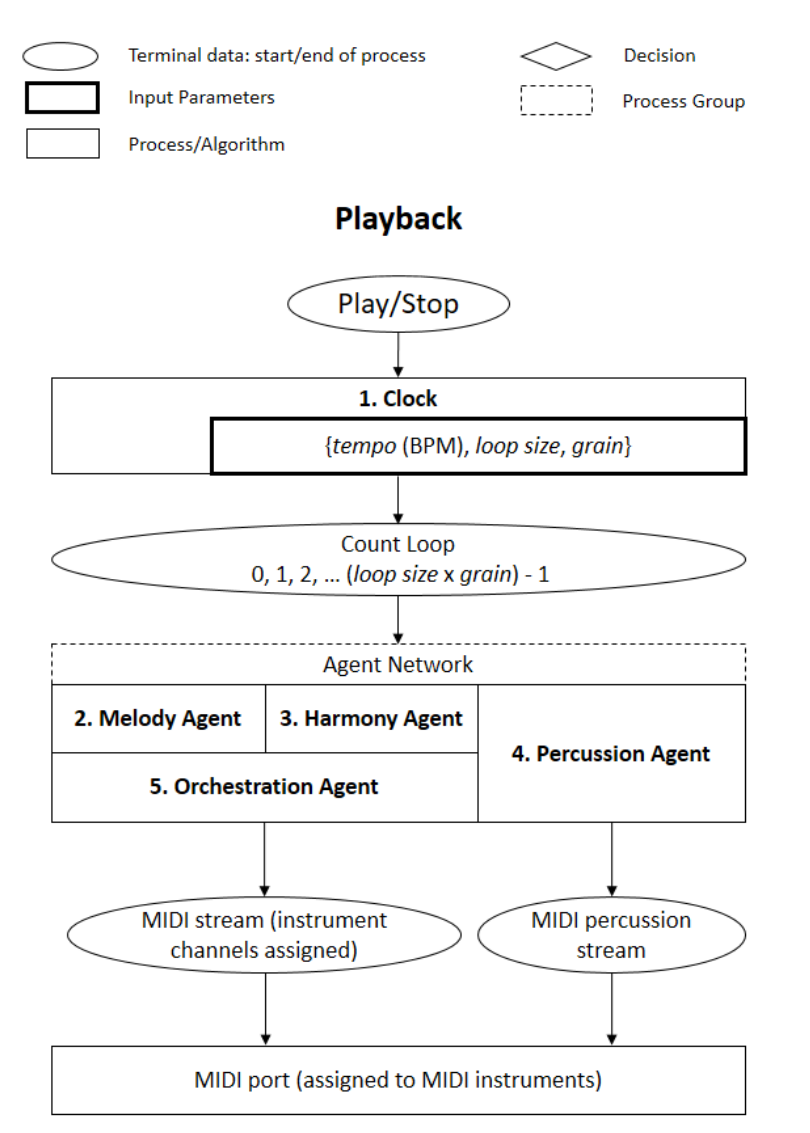
\includegraphics[width=\linewidth,height=10cm]{images/pamg_algorithm.png}
    \caption{Algorithm / architecture of PAMG \cite{lopez2023progressive}}
    \label{fig:pamg_algorithm}
\end{figure}


\subsubsection{Melody Agent}

\subsubsection{Harmony Agent}

\subsubsection{Percussion Agent}

\subsubsection{Orcestration Agent}